\documentclass[12pt]{article}
\usepackage{amsmath}
\usepackage{amssymb}
\usepackage{geometry}
\usepackage{enumerate}
\usepackage{natbib}
\usepackage{float}%稳定图片位置
\usepackage{graphicx}%画图
\usepackage[english]{babel}
\usepackage{a4wide}
\usepackage{indentfirst}%缩进
\usepackage{enumerate}%加序号
\usepackage{multirow}%合并行
\title{\large UM-SJTU JOINT INSTITUTE\\PHYSICS LABTORATORY\\(VP241)\\\ \\\ \\\ \\\ \\\ \\\ \\\ \\\ \\\ \\\ \\\
LABTORATORY REPORT\\\ \\\ EXERCISE 2\\\ The Hall Probe: Characteristics and Applications
This lab \\\ \\\ \\\ \\\ \\\ }
\author{Name: Pan Chongdan \\ID: 516370910121\\Partner:DelmwinBaeka\\ID:516370990007\\Group: 6}
\date{Date: \today}

\begin{document}
\maketitle
\newpage
\section{Objectives}
\begin{enumerate}
\item Study the principle of the Hall effect and its applications by using a Hall probe.
\item Verify that Hall voltage is proportional to the magnetic field.
\item Study the sensitivity of an integrated Hall probe by calculating the magnetic field at the center of a solenoid.
\item Measure the distribution of the magnetic field along the axis of the solenoid and compare it with the corresponding theoretical curve. 
\end{enumerate}
\section{Introduction and Theoretical Background}
\subsection{Hall Effect}
Consider a conducting sheet (made of a metal or a semiconductor) placed in a magnetic
field so that the plane of the sheet is perpendicular to the direction of the magnetic field $B$. When the electric current $I$ passes through the sheet in the direction shown
in Figure 1, an electric potential difference between the sides $a$ and $b$ of the sheet is
generated. The corresponding electric field is perpendicular to both the direction of the
current and the direction of the magnetic field. This effect is known as the Hall effect,
and the electric potential difference is called the Hall voltage $U_H$.
\begin{figure}[H]
\centering
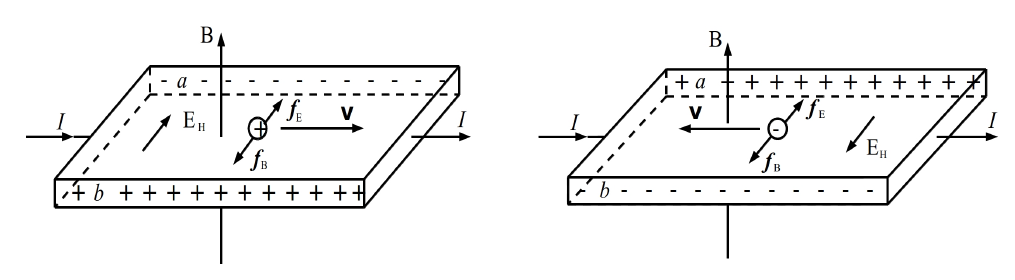
\includegraphics[scale=0.3]{P1.jpg}
\caption{The principle of Hall effect}
\end{figure}
Microscopically, the Hall effect is caused by the Lorentz force, that is a force acting on
charges moving in a magnetic field. The Lorentz force $F_B$ leads to the detection of the
moving charges, and their accumulation on one side of the sheet, which in turn increases
the magnitude of the transverse electric field $E_H$ (the Hall field). Due to this field, there
is an electric force $F_E$ acting upon the charges, and since $F_B$ and $F_E$ act in opposite
directions, a balance is eventually reached and $U_H$ stabilizes. The sign of UH depends on
the sign of the charge carriers (positive or negative). Therefore the type of charge carriers
in semiconductors can be determined by analyzing the sign of $U_H$.
\par When the external magnetic field is not too strong, the Hall voltage is proportional
to both the current and the magnitude of the magnetic field, and inversely proportional
to the thickness of the sheet $d$
\begin{equation}
U_H=R_H\frac{IB}{d}=KIB
\end{equation}
where $R_H$ is the so-called Hall coefficient and $K=R_H/d=K_H/I$, where $K_H$ is the so-called sensitivity of the Hall element.
\subsection{Integrated Hall Probe}
The magnitude of the magnetic field can be found by measuring the Hall voltage with a
Hall probe when the sensitivity $K_H$ and the current $I$ are fixed. Since the Hall voltage is
usually very small, it should be amplified before the measurement.
\par Silicon can be used to design both the Hall probe and the integrated circuits, so it is
convenient to arrange the Hall probe and the electric circuits into a single device. Such a
device is called an integrated Hall probe.
\par The integrated Hall probe SS495A consists of a Hall sensor, an amplifier, and a voltage
compensator (Figure 2). The output voltage $U$ can be read ignoring the residual voltage.
The working voltage $U_S$ = $5V$, and the output voltage $U_0$ is approximately 2.5 $V$ when
the magnetic field is zero. The relation between the output voltage $U$ and the magnitude
of the magnetic field is 
\begin{equation}
B=\frac{U-U_0}{K_H}
\end{equation}
\begin{figure}[H]
\centering
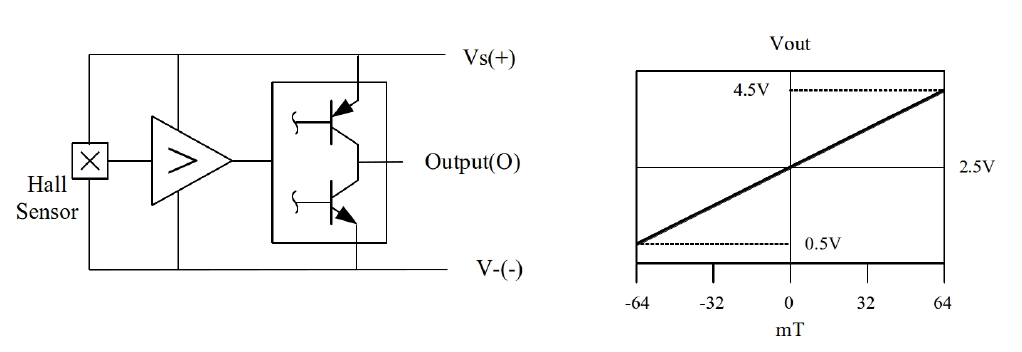
\includegraphics[scale=0.4]{P2.jpg}
\caption{The integrated Hall probe SS495A (left). The relation between the output
voltage $U$ and the magnitude of the magnetic field $B$ (right).}
\end{figure}
\subsection{Magnetic Field Distribution Inside a Solenoid}
The magnetic field distribution on the axis of a single layer solenoid can be calculated
from the following formula
\begin{equation}
B(x)=\mu_0\frac{N}{L}I_M\left\{\frac{L+2x}{2[D^2+(L+2x)^2]^\frac{1}{2}}+\frac{L-2x}{2[D^2+(L-2x)^2]^\frac{1}{2}}1\right\}
\end{equation}
where $N$ is the number of turns of the solenoid, $L$ is its length, $I_M$ is the current through the solenoid wire, and $D$ is the solenoid's diameter. The magnetic permeability of vacuum is $\mu_0=4\pi\cdot10^7H/m$.
\par The solenoid used in this exercise has ten layers, and the magnetic field $B(x)$ for
each layer can be calculated using Eq. (3). Then the net magnetic on the axis of the
solenoid can be found by adding contributions due to all layers. The theoretical value of
the magnetic field inside the solenoid with $I_M = 0:1 A$ is given in Table 1.
\begin{table}[H]
\centering
\begin{tabular}{|c|c|c|c|}
\hline
x[cm] & B[mT]  & X[cm] & B[mT]  \\ \hline
$\pm0.0$   	  & 1.4366 &$\pm8.0$       & 1.4057 \\ \hline
$\pm1.0$ 	  & 1.4363 &$\pm9.0$       & 1.3856 \\ \hline
$\pm2.0$      & 1.4356 &$\pm10.0$       & 1.3478 \\ \hline
$\pm3.0$      & 1.4343 &$\pm11.0$       & 1.2685 \\ \hline
$\pm4.0$      & 1.4323 &$\pm11.5$       & 1.1963 \\ \hline
$\pm5.0$      & 1.4292 &$\pm12.0$      & 1.0863 \\ \hline
$\pm6.0$      & 1.4245 &$\pm12.5$       & 0.9261 \\ \hline
$\pm7.0$      & 1.4173 &$\pm13.0$       & 0.7233 \\ \hline
\end{tabular}
\caption{Theoretical value of the magnetic field inside the solenoid.}
\end{table}
\subsection{Study of the Geomagnetic Field with a Hall Probe}
The geomagnetic field is the magnetic associated with the Earth. The geomagnetic field
lines are shown schematically in Figure 3. The Earth's magnetic field is similar to that of
a bar magnet tilted about $11.5^o$ degrees from the spin axis of the Earth.
\begin{figure}[H]
\centering
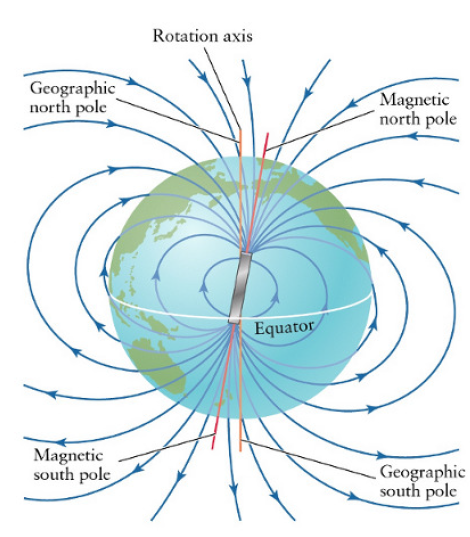
\includegraphics[scale=0.4]{P3.jpg}
\caption{Magnetic field of the Earth.}
\end{figure}
\par Figure 4 shows the geomagnetic field distribution of China in 1970. The magnetic
inclination is about $44:5^o$ and the magnitude of the magnetic field in Shanghai is about
48000 nT.
\begin{figure}[H]
\centering
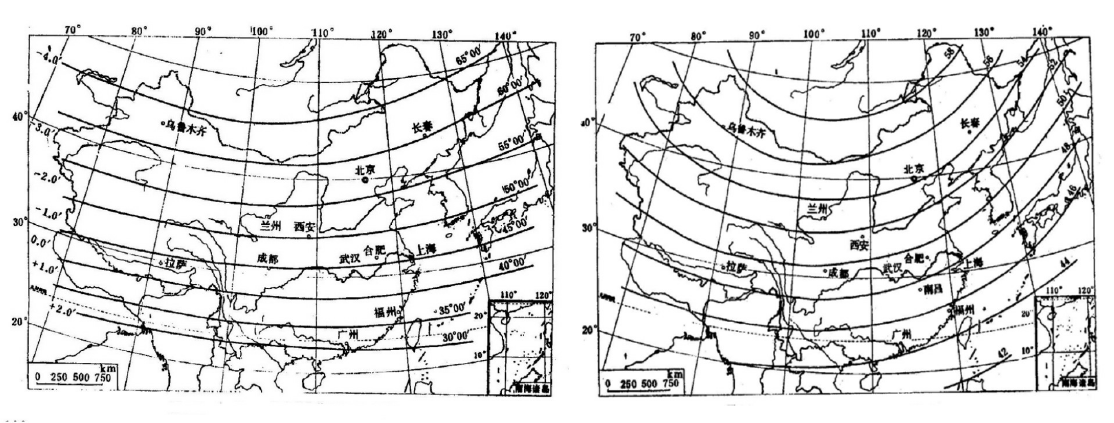
\includegraphics[scale=0.4]{P4.jpg}
\caption{Geomagnetic inclination in China, 1970 (left). The magnitude of the geomagnetic field in China, 1970 (right).}
\end{figure}
\section{Apparatus}
The experimental setup shown in Figure 5 consists of an integrated Hall probe SS495A
(see Figure 6) with $K_H = 31.25\pm1.25V/T$ or $K_H=3.125\pm0.125mV/G$, a solenoid, a
power supply, a voltmeter, a DC voltage divider, and a set of connecting wires.
\begin{figure}[H]
\centering
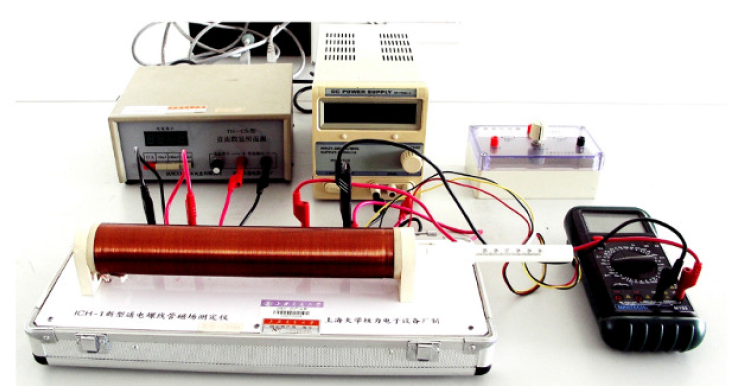
\includegraphics[scale=0.4]{P5.jpg}
\caption{Measurement setup.}
\end{figure}
\begin{figure}[H]
\centering
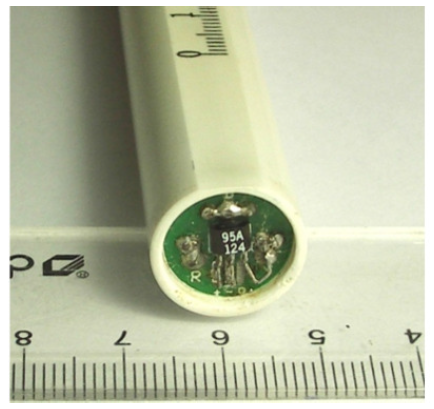
\includegraphics[scale=0.4]{P6.jpg}
\caption{Integrated Hall probe SS495A.}
\end{figure}
\section{Procedure}
\subsection{Relation between Sensitivity $K_H$ and Working Voltage $U_S$}
\begin{enumerate}
\item I placed the integrated Hall probe at the center of the solenoid and set the working voltage at $5V$ to measure the output voltage $U_0(I_M=0)$ and $U(I_M=250mA)$. Then I take the theoretical value of $B(x = 0)$ from Table 1 and calculate the sensitivity of the probe $K_H$ by using Eq. (2).
\item I measured $K_H$ for different values of $U_S$ from 2.8 V to 10 V and calculate $K_H=U_S$ to plot the curve $K_H=U_S$ vs. $U_S$.
\end{enumerate}
\subsection{Relation between Output Voltage $U$ and Magnetic field $B$}
\begin{enumerate}
\item I connected the $2.4\sim2.6V$ output terminal of the DC voltage
divider and the negative port of the voltmeter with $B=0$, $U_S=5V$, then adjust the voltage until $U_0=0$.
\item I placed the integrated Hall probe at the center of the solenoid and measured the output
voltage $U$ for different values of $I_M$ ranging from 0 to 500 $mA$, with intervals of $50
mA$.
\item I explain the relation between $B(x=0)$ and the Hall voltage $U_H$ in the report by using output voltage $U$ as amplified signal from $U_H$ and the theoretical
value of $B(x = 0)$ from Table 1.
\item Then I plot the curve $U$ vs. $B$ to find the sensitivity $K_H$ by a linear fit and compare the value  with the theoretical value in given in the Apparatus
section.
\end{enumerate}
\subsection{Magnetic Field Distribution Inside the Solenoid}
\begin{enumerate}
\item I measure the magnetic field distribution along the axis of the solenoid for $I_M=250
mA$, record the output voltage $U$ and the corresponding position $x$. Then find $B = B(x)$. (Use the value of $K_H$ found in the previous part of the experiment).
\item I plot the theoretical and the experimental curve showing the
magnetic field distribution inside the solenoid by using dots for the data measured and
a solid line for the theoretical curve. The origin of the plot is at the center
of the solenoid.
\end{enumerate}
\subsection{Measurement of the Geomagnetic Field}
I used the integrated Hall probe to measure the magnitude and the direction of the
geomagnetic field.
\section{Results \& Calculations}
\subsection{$U_0$ and U with $U_S$=5V}
\subsubsection{Measured Data for $U_0$ and U with $U_S$=5V}
\begin{table}[H]
\centering
\begin{tabular}{|c|c|c|}
\hline
$U_S\pm0.05\%[V]$ &$U_0(I_M=0mA)\pm0.05\%+6\cdot10^{-3}[V]$  &$U_0(I_M=250mA)\pm0.05\%+6\cdot10^{-3}[V]$  \\ \hline
4.99&2.479&2.584  \\ \hline
\end{tabular}
\end{table}
\subsubsection{Calculation for $K_H$}
$$K_H=\frac{U-U_0}{B}=\frac{2.584-2.479}{1.4366\cdot10^{-3}}=73.90\pm7.15[V/T]$$
\subsubsection{Relation between Sensitivity $K_H$ and Working Voltage $U_S$}
\begin{table}[H]
\centering
\begin{tabular}{|c|c|c|c|c|c|}
\hline
&$U_S\pm0.05\%[V]$   &$U_0\pm0.05\%+6\cdot10^{-3}[V]$&$U\pm0.05\%+6\cdot10^{-3}[V]$&$K_H[V/T]$   &$K_H/U_S[1/T]$\\ \hline
1&2.8    &1.452  &1.492&27.84&9.94  \\ \hline
2 &3.2   &1.572  &1.627&38.28&11.96  \\ \hline
3 &3.6   &1.772  &1.854&57.08&15.86  \\ \hline
4 &4.0   &1.982  &2.062&55.69&13.92  \\ \hline
5 &4.4   &2.178  &2.278&69.61&15.89  \\ \hline
6 &4.8   &2.379  &2.479&69.61&14.50  \\ \hline
7 &5.2   &2.580  &2.694&79.35&15.26  \\ \hline
8 &5.6   &2.778  &2.894&80.75&14.42  \\ \hline
9 &6.0   &2.981  &3.109&89.10&14.85  \\ \hline
10 &6.4  &3.175  &3.320&100.9&15.77  \\ \hline
11 &6.8  &3.377  &3.530&106.5&15.66  \\ \hline
12 &7.2  &3.586  &3.743&109.3&15.18  \\ \hline
13 &7.6  &3.781  &3.943&112.8&14.84  \\ \hline
14 &8.0  &3.987  &4.150&113.5&14.19  \\ \hline
15 &8.4  &4.178  &4.363&128.8&15.33  \\ \hline
16 &8.8  &4.384  &4.574&132.3&15.03  \\ \hline
17 &9.2  &4.576  &4.781&142.7&15.51  \\ \hline
18 &9.6  &4.784  &4.989&142.7&14.86  \\ \hline
19 &10.0 &4.979  &5.189&146.2&14.62  \\ \hline
\end{tabular}
\caption{Data of $K_H$ for $U_0$ and $U$ with different $U_S$}
\end{table}
\subsubsection{Plot of Sensitivity $K_H/U_S$ and Working Voltage $U_S$}
\begin{figure}[H]
\centering
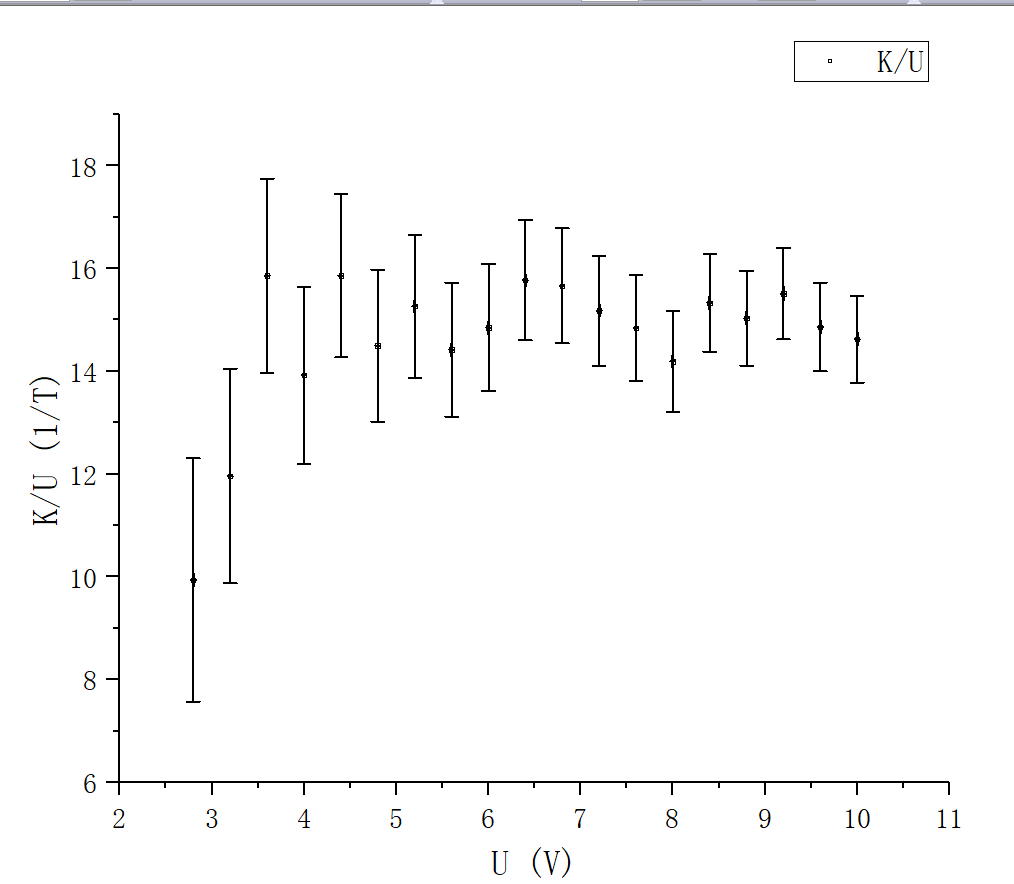
\includegraphics[scale=0.25]{P7.jpg}
\end{figure}
\subsection{$I_M$ vs. $U$ relation}
\begin{table}[H]
\centering
\begin{tabular}{|c|c|c|}
\hline
  &$I_M\pm2\%[mA]$&$U\pm0.05\%+6\cdot 10^{-4}[V]$  \\ \hline
1 &0    &0.0000  \\ \hline
2 &50   &0.0211  \\ \hline
3 &100  &0.0418  \\ \hline
4 &150  &0.0624  \\ \hline
5 &200  &0.0832  \\ \hline
6 &250  &0.1039  \\ \hline
7 &300  &0.1251  \\ \hline
8 &350  &0.1453  \\ \hline
9 &400  &0.1661  \\ \hline
10&450  &0.1871  \\ \hline
11&500  &0.2080  \\ \hline
\end{tabular}
\end{table}
\subsubsection{Calculation of $B$}
$$B(x)=C(x)I_M$$
$$C(0)=\frac{B(0)}{I_M}=\frac{1.436\cdot10^{-3}}{0.1}=1.4366\cdot10^{-2}[T/A]$$
\begin{table}[H]
\centering
\begin{tabular}{|c|c|c|}
\hline
  &$B[T]$&$U[V]$  \\ \hline
1 &0    &0.0000  \\ \hline
2 &$7.184\cdot10^{-4}$   &0.0211  \\ \hline
3 &$1.437\cdot10^{-3}$  &0.0418  \\ \hline
4 &$2.155\cdot10^{-3}$  &0.0624  \\ \hline
5 &$2.873\cdot10^{-3}$  &0.0832  \\ \hline
6 &$3.592\cdot10^{-3}$  &0.1039  \\ \hline
7 &$4.310\cdot10^{-3}$  &0.1251  \\ \hline
8 &$5.028\cdot10^{-3}$  &0.1453  \\ \hline
9 &$5.746\cdot10^{-3}$  &0.1661  \\ \hline
10&$6.465\cdot10^{-3}$  &0.1871  \\ \hline
11&$7.183\cdot10^{-3}$  &0.2080  \\ \hline
\end{tabular}
\caption{Relation between $B$ and $U$}
\end{table}
\subsubsection{Plot for relation between $B$ and $U$}
\begin{figure}[H]
\centering
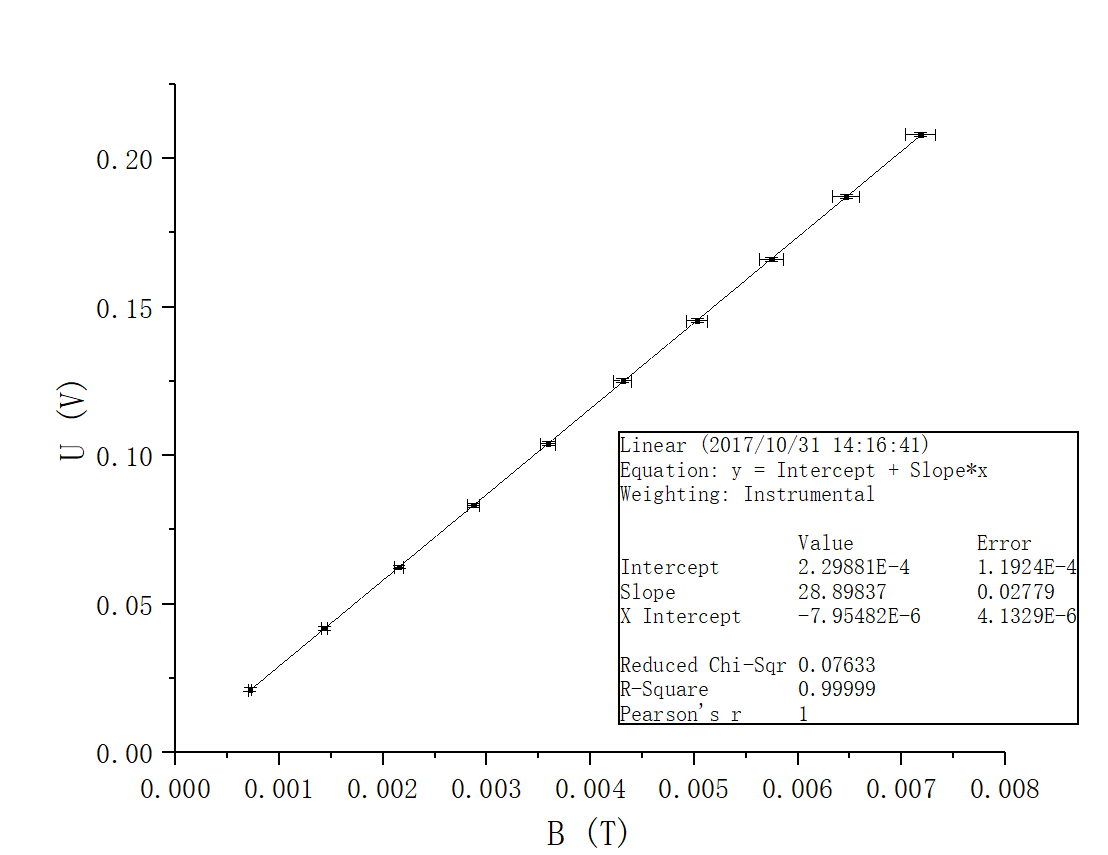
\includegraphics[scale=0.4]{P8.jpg}
\end{figure}
$U_H$ becomes bigger as $B$ increasing, and they're proportional to each other.
According to linear fit, the slope $K_H$ is $28.8983\pm0.0277$, which is a little smaller than the value in apparatus section.
\subsection{$U$ vs. $x$ relation}
\subsubsection{Measured Data for $x$ and $U$}
\begin{table}[H]
\centering
\begin{tabular}{|c|c|c||c|c|c|}
\hline
   &$x\pm0.05[cm]$&$U\pm0.05\%+6\cdot10^{-4}[V]$&  &$x\pm0.05[cm]$&$U\pm0.05\%+6\cdot10^{-4}[V]$  \\ \hline
1  & 0.0 &0.0485  &27  &15.6  &0.1050  \\ \hline
2  & 0.6 &0.0679  &28  &16.2  &0.1050  \\ \hline
3  & 1.2 &0.0793  &29  &16.8  &0.1048  \\ \hline
4  & 1.8 &0.0893  &30  &17.4  &0.1047  \\ \hline
5  & 2.4 &0.0944  &31  &18.0  &0.1045  \\ \hline
6  & 3.0 &0.0975  &32  &18.6  &0.1045  \\ \hline
7  & 3.6 &0.0996  &33  &19.2  &0.1039  \\ \hline
8  & 4.2 &0.1019  &34  &19.8  &0.1035  \\ \hline
9  & 4.8 &0.1025 &35  &20.4  &0.1031  \\ \hline
10 & 5.4 &0.1028  &36  &21.0 &0.1024  \\ \hline
11 & 6.0 &0.1034  &37  &21.6  &0.1015  \\ \hline
12 & 6.6 &0.1037  &38  &22.2  &0.0999  \\ \hline
13 & 7.2 &0.1040  &39  &22.8 &0.0973  \\ \hline
14 & 7.8 &0.1043  &40  &23.4  &0.0958  \\ \hline
15 & 8.4 &0.1044  &41  &24.6  &0.0897  \\ \hline
16 & 9.0 &0.1046  &42  &25.2  &0.0823  \\ \hline
17 & 9.6 &0.1047  &43  &25.8  &0.0730  \\ \hline
18 & 10.2 &0.1047  &44 &26.4  &0.0548  \\ \hline
19 & 10.8 &0.1046  &45 &27.0  &0.0377  \\ \hline
20 & 11.4 &0.1046  &46 &27.6 &0.0147  \\ \hline
21 & 12.0 &0.1046  &47 &28.2  &0.0088  \\ \hline
22 & 12.6 &0.1047  &48 &28.8  &0.0050  \\ \hline
23 & 13.2 &0.1048  &49 &  &  \\ \hline
24 & 13.8 &0.1049  &50 &  &  \\ \hline
25 & 14.4 &0.1049  &51 &  &  \\ \hline
26 & 15.0 &0.1050  &52 &  &  \\ \hline
\end{tabular}
\end{table}
\subsubsection{Calculation for $B(x)$}
$$B(x)=\frac{U}{K_H}$$
$$B(0)=\frac{0.0485}{28.898}=1.678\cdot10^{-3}[T]$$
\begin{table}[H]
\centering
\begin{tabular}{|c|c|c||c|c|c|}
\hline
   &$x\pm0.05[cm]$&$B[T]$&  &$x\pm0.05[cm]$&$B[T]$  \\ \hline
1  & 0.0 &$1.678\cdot10^{-3}$  &27  &15.6  &$3.633\cdot10^{-3}$  \\ \hline
2  & 0.6 &$2.350\cdot10^{-3}$  &28  &16.2  &$3.633\cdot10^{-3}$  \\ \hline
3  & 1.2 &$2.744\cdot10^{-3}$  &29  &16.8  &$3.627\cdot10^{-3}$  \\ \hline
4  & 1.8 &$3.090\cdot10^{-3}$  &30  &17.4  &$3.623\cdot10^{-3}$  \\ \hline
5  & 2.4 &$3.267\cdot10^{-3}$  &31  &18.0  &$3.616\cdot10^{-3}$  \\ \hline
6  & 3.0 &$3.374\cdot10^{-3}$  &32  &18.6  &$3.616\cdot10^{-3}$  \\ \hline
7  & 3.6 &$3.447\cdot10^{-3}$  &33  &19.2  &$3.595\cdot10^{-3}$  \\ \hline
8  & 4.2 &$3.526\cdot10^{-3}$  &34  &19.8  &$3.582\cdot10^{-3}$  \\ \hline
9  & 4.8 &$3.526\cdot10^{-3}$ &35  &20.4  &$3.568\cdot10^{-3}$  \\ \hline
10 & 5.4 &$3.557\cdot10^{-3}$  &36  &21.0 &$3.543\cdot10^{-3}$  \\ \hline
11 & 6.0 &$3.578\cdot10^{-3}$  &37  &21.6  &$3.512\cdot10^{-3}$  \\ \hline
12 & 6.6 &$3.588\cdot10^{-3}$  &38  &22.2  &$3.457\cdot10^{-3}$  \\ \hline
13 & 7.2 &$3.599\cdot10^{-3}$  &39  &22.8 &$3.367\cdot10^{-3}$  \\ \hline
14 & 7.8 &$3.609\cdot10^{-3}$  &40  &23.4  &$3.315\cdot10^{-3}$  \\ \hline
15 & 8.4 &$3.612\cdot10^{-3}$  &41  &24.6  &$3.104\cdot10^{-3}$  \\ \hline
16 & 9.0 &$3.620\cdot10^{-3}$  &42  &25.2  &$2.848\cdot10^{-3}$  \\ \hline
17 & 9.6 &$3.623\cdot10^{-3}$  &43  &25.8  &$2.526\cdot10^{-3}$ \\ \hline
18 & 10.2 &$3.623\cdot10^{-3}$  &44 &26.4  &$1.896\cdot10^{-3}$  \\ \hline
19 & 10.8 &$3.620\cdot10^{-3}$ &45 &27.0  &$1.305\cdot10^{-3}$  \\ \hline
20 & 11.4 &$3.620\cdot10^{-3}$ &46 &27.6 &$3.568\cdot10^{-4}$  \\ \hline
21 & 12.0 &$3.620\cdot10^{-3}$  &47 &28.2  &$5.087\cdot10^{-4}$  \\ \hline
22 & 12.6 &$3.623\cdot10^{-3}$  &48 &28.8  &$1.730\cdot10^{-4}$  \\ \hline
23 & 13.2 &$3.627\cdot10^{-3}$  &49 &  &  \\ \hline
24 & 13.8 &$3.630\cdot10^{-3}$  &50 &  &  \\ \hline
25 & 14.4 &$3.630\cdot10^{-3}$  &51 &  &  \\ \hline
26 & 15.0 &$3.633\cdot10^{-3}$  &52 &  &  \\ \hline
\end{tabular}
\end{table}
\subsubsection{Theoretical Value of B when $I=250mA$ }
$B'=\frac{B\cdot0.25}{0.1}=1.4366\cdot2.5=3.5915[mT]$
\begin{table}[H]
\centering
\begin{tabular}{|c|c|c|c|}
\hline
x[cm] & B[mT]  & X[cm] & B[mT]  \\ \hline
$\pm0.0$   	  & 3.5915 &$\pm8.0$       & 3.5143 \\ \hline
$\pm1.0$ 	  & 3.5908 &$\pm9.0$       & 3.464 \\ \hline
$\pm2.0$      & 3.589 &$\pm10.0$       & 3.3695 \\ \hline
$\pm3.0$      & 3.5858 &$\pm11.0$       & 3.1713 \\ \hline
$\pm4.0$      & 3.5808 &$\pm11.5$       & 2.9908 \\ \hline
$\pm5.0$      & 3.573 &$\pm12.0$      & 2.7158 \\ \hline
$\pm6.0$      & 3.5613 &$\pm12.5$       & 2.3153 \\ \hline
$\pm7.0$      & 3.5433 &$\pm13.0$       & 1.8083 \\ \hline
\end{tabular}
\caption{Theoretical value of the magnetic field inside the solenoid.}
\end{table}
\subsection{Plot of Magnetic field inside the Solenoid}
The black line is the theoretical value and red dots are measured value.
\begin{figure}[H]
\centering
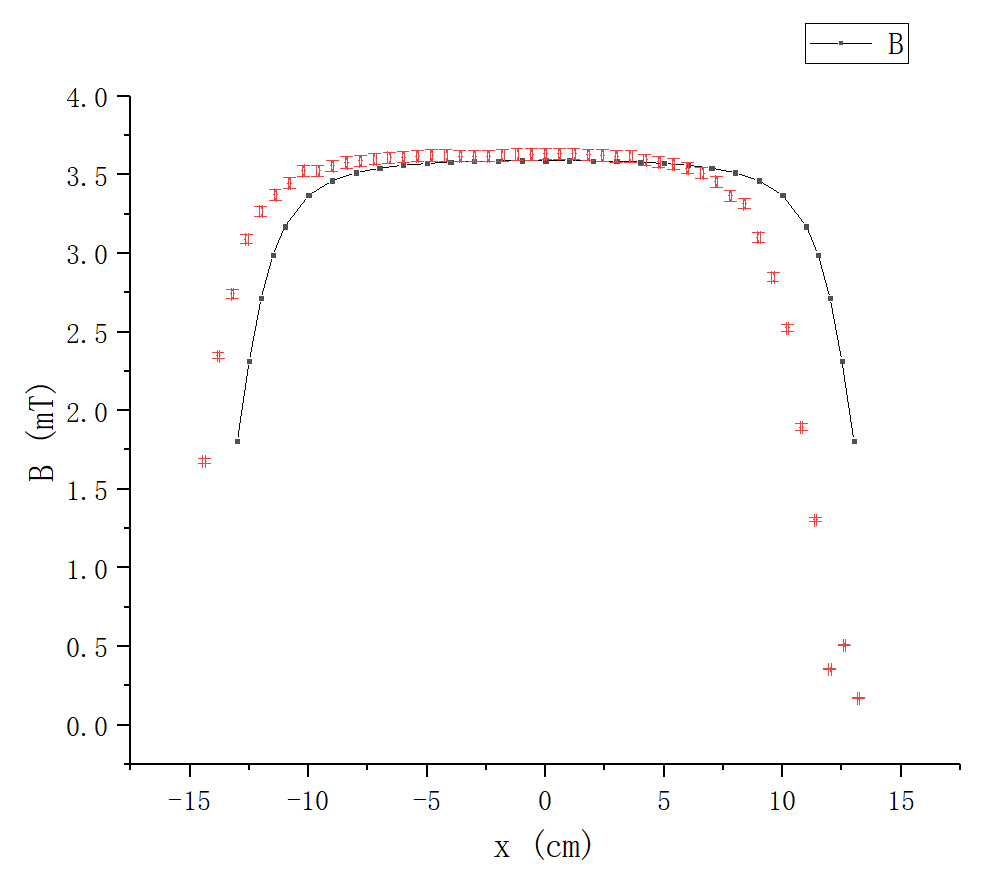
\includegraphics[scale=0.4]{P9.jpg}
\end{figure}
\section{Uncertainty Analysis}
\subsection{Uncertainty for Relation between Sensitivity $K_H$ and Working Voltage $U_S$}
when $U_S=5V$:
$$u=\sqrt{(\frac{\partial K_H}{\partial U_0}\cdot u_0)^2+(\frac{\partial K_H}{\partial U}\cdot u_u)^2}=7.15[V/T]$$
$$u_r=\frac{u}{K_H}\cdot100\%=9.68\%$$
The uncertainty for $u=\sqrt{(\frac{u_K}{u})^2+(\frac{K}{u^2}\cdot u_u)^2}=2.3679[1/T]$
\begin{table}[H]
\centering
\begin{tabular}{|c|c|c|c|c|c|}
\hline
&$U_S\pm0.05\%[V]$&$K_H[V/T]$&$u_K[V/T]$&$u_r\%$&$u[1/T]$   \\ \hline
1&2.8    &27.84&6.63&23.81&2.3679  \\ \hline
2 &3.2   &38.28&6.69&17.48&2.0906  \\ \hline
3 &3.6   &57.08&6.80&11.91&1.8889  \\ \hline
4 &4.0   &55.69&6.90&12.39&1.725  \\ \hline
5 &4.4   &69.61&7.00&10.06&1.5909  \\ \hline
6 &4.8   &69.61&7.10&10.20&1.4792  \\ \hline
7 &5.2   &79.35&7.20&9.07 &1.3846 \\ \hline
8 &5.6   &80.75&7.30&9.04 &1.3036 \\ \hline
9 &6.0   &89.10&7.40&8.31 &1.2334 \\ \hline
10 &6.4  &100.9&7.50&7.43 &1.1719 \\ \hline
11 &6.8  &106.5&7.60&7.14 &1.1177 \\ \hline
12 &7.2  &109.3&7.70&7.04 &1.0695 \\ \hline
13 &7.6  &112.8&7.80&6.91 &1.0263 \\ \hline
14 &8.0  &113.5&7.90&6.96 &0.9875 \\ \hline
15 &8.4  &128.8&8.00&6.21 &0.9524 \\ \hline
16 &8.8  &132.3&8.11&6.13 &0.9216 \\ \hline
17 &9.2  &142.7&8.21&5.75 &0.8924 \\ \hline
18 &9.6  &142.7&8.31&5.82 &0.8657 \\ \hline
19 &10.0 &146.2&8.41&5.75 &0.841 \\ \hline
\end{tabular}
\caption{Data of $K_H$ for $U_0$ and $U$ with different $U_S$}
\end{table}
\subsection{Uncertainty for Relation between $I_M$ vs. $U$}
$$B=C(0)I_M$$
$$u_B=C(0)\cdot u_I=1.4366\cdot10^{-2}\cdot50\cdot10^{-3}\cdot2\%=1.4366\cdot10^{-5}[T]$$
$$u_r=\frac{u_B}{B}\cdot100\%=2.00\%$$
$$u_v=0.0211\cdot0.05\%+6\cdot10^{-4}=6.1055\times10^{-4}$$
$$u_r=\frac{6.1055\times10^{-4}}{0.0211}\cdot100\%=2.89\%$$
\begin{table}[H]
\centering
\begin{tabular}{|c|c|c|c|c|c|c|}
\hline
  &$B[T]$&$u_B[T]$&$u_r[\%]$&$U[V]$&$u_v[V]$&$u_r[\%]$  \\ \hline
1 &0&0&0    &0.0000&0&0  \\ \hline
2 &$7.184\cdot10^{-4}$&$1.4366\cdot10^{-5}$&$2.00$&0.0211&$6.106\cdot10^{-4}$&2.89  \\ \hline
3 &$1.437\cdot10^{-3}$&$2.8732\cdot10^{-5}$&$2.00$  &0.0418&$6.209\cdot10^{-4}$&1.49  \\ \hline
4 &$2.155\cdot10^{-3}$&$4.3098\cdot10^{-5}$&$2.00$  &0.0624&$6.312\cdot10^{-4}$&1.01  \\ \hline
5 &$2.873\cdot10^{-3}$&$5.7464\cdot10^{-5}$&$2.00$  &0.0832&$6.416\cdot10^{-4}$&0.77  \\ \hline
6 &$3.592\cdot10^{-3}$&$7.183\cdot10^{-5}$&$2.00$   &0.1039&$6.520\cdot10^{-4}$&0.63  \\ \hline
7 &$4.310\cdot10^{-3}$&$8.6196\cdot10^{-5}$&$2.00$  &0.1251&$6.626\cdot10^{-4}$&0.53  \\ \hline
8 &$5.028\cdot10^{-3}$&$1.0056\cdot10^{-4}$&$2.00$  &0.1453&$6.727\cdot10^{-4}$&0.46  \\ \hline
9 &$5.746\cdot10^{-3}$&$1.1493\cdot10^{-4}$&$2.00$  &0.1661&$6.831\cdot10^{-4}$&0.41  \\ \hline
10&$6.465\cdot10^{-3}$&$1.2929\cdot10^{-4}$&$2.00$  &0.1871&$6.936\cdot10^{-4}$&0.37  \\ \hline
11&$7.183\cdot10^{-3}$&$1.4366\cdot10^{-4}$&$2.00$  &0.2080&$7.04\cdot10^{-4}$&0.34 \\ \hline
\end{tabular}
\caption{Uncertainty for relation between $B$ and $U$}
\end{table}
\subsection{Uncertainty for Relation between $B$ and $x$}
$$u_B=\sqrt{(\frac{u_u}{K_H})^2+(\frac{U\cdot u_K}{K_H^2})^2}=1.609\cdot10^{-6}[T]$$
$$u_r=\frac{u_B}{B}\cdot100\%=0.1\%$$
\section{conclusion}
In this exercise, I studied Hall effect by using an Integrated Hall Probe, which can show the magnitude of the magnetic field indirectly through the Hall voltage. 
\par First, I measure the voltage when $U_S=5V$ and get the sensitivity of the Hall element $K_H=73.90\pm7.15[V/T]$. It's relative uncertainty is 9.68$\%$ is quite big, I think it's because $B$ is so small that the uncertainty of voltage is amplified.
\par Second, I calculated $K_H$ at different $U_S$ and plot the figure. At first, $K_H/U_S$ increase greatly as $U_S$ becomes bigger, and then it doesn't change very much. The uncertainty for it is also very big, I think it's the same reason in last paragraph.
\par Third, I measured $B$ indirectly by measuring $I_M$ when $x=13cm$. I get another $K_H$,which is the slope of linear fit plot of $U$ vs. $B$ and $K_H=28.28983\pm0.0277[V/T]$, which is a bit smaller than the given value of $31.25\pm1.25[V/T]$ from the apparatus section. The relative uncertainty is very small, I think it's due to some measurement error. 
\par At last, I used the $K_H$ which I have got to calculate $B$ at different x in the solenoid by measuring the voltage. I measured more than 40 values to make my plot more accurate, and it's similar to the theoretical line. However, in my plot, my measured dots is on the left side of the theoretical line, I think it's because I didn't know the center of the solenoid when I measuring the voltage.
\par Due to the time limit, I didn't measure the Geomagnetic field through Hall probe but I still learnt a lot from the lab manual about the Geomagnetic field.
\subsection{Suggestions and Improvement}
\begin{enumerate}
\item I should first find out where the center of solenoid is before measuring the voltage
\item The accuracy of the measurement setup is so big that there is a high uncertainty in first part. I think it should be improved.
\end{enumerate}

\section{Data Sheet}
Data sheet is attach to the report
\section{Reference}
\par Young, H.D., Freedman R.A. University Physics. Chapter 28,31.
\par Krzyzosiak,M. Lab Manual of Exercise 2.
\par Qin Tian, Zeng Ming, Zhao Xijian, Krzyzosiak,M. Handbook-Uncertainty Analysis.
\end{document}